\chapter{Background}  

The study of quantum automata theory necessitates a thorough grounding in both classical computational models and the quantum mechanical principles that redefine their capabilities. This chapter systematically establishes the conceptual foundation for analyzing quantum automata by first revisiting classical finite automata—the cornerstone of formal language theory—and then introducing the quantum mechanical framework that enables novel computational paradigms.

We begin with an in-depth exploration of classical finite automata, which serve as the theoretical bedrock for understanding computational limits and language recognition. \glspl{dfa}, \glspl{nfa}, \glspl{pfa}, and their two-way variants are analyzed through their formal definitions, operational dynamics, and closure properties. These models collectively define the boundaries of classical computation, particularly in recognizing regular languages and their limitations in handling context-free or stochastic languages. The analysis draws on foundational works such as Hopcroft et al. \cite{hopcroft2006introduction}, which formalized the equivalence between \glspl{dfa} and \glspl{nfa}, and Rabin's seminal work on probabilistic automata \cite{rabin1963probabilistic}, which expanded the class of recognizable languages through probabilistic acceptance criteria.

The discourse then transitions to quantum mechanical principles essential for quantum computation. Key concepts such as qubit representation, quantum superposition, and entanglement are contextualized within computational frameworks, emphasizing their departure from classical bit-based processing. The measurement postulate and its implications for probabilistic outcomes are discussed in relation to quantum state collapse—a critical distinction from classical probabilistic models. These principles are synthesized with insights from Nielsen and Chuang's definitive text on quantum computation \cite{nielsen2010quantum}, which provides the mathematical formalism for quantum operations.

The chapter's structure is designed to mirror the hierarchical taxonomy developed in later chapters. By first rigorously defining classical models and their limitations, followed by an exposition of quantum principles and their computational implications, the groundwork is laid for analyzing hybrid models such as the \gls{1qfac} \cite{zheng2012one}. Each section deliberately connects theoretical constructs to practical considerations, such as the role of decoherence in open quantum systems \cite{breuer2002theory} and its impact on automata design. This approach ensures that subsequent discussions of quantum automata variants are rooted in both mathematical rigor and physical realizability.

\section{Classical Finite Automata}
\label{sec:classical-finite-automata} 

Finite automata form the cornerstone of formal language theory, providing mathematical frameworks to analyze computational limits and language recognition capabilities. This section systematically examines deterministic, nondeterministic, probabilistic, and two-way variants, emphasizing their structural relationships and computational boundaries. 


\subsection{Shared Foundations}
\label{subsec:shared-foundations} 

The study of automata begins with foundational concepts in formal language theory, pioneered by figures such as Stephen Kleene \cite{kleene1956representation}, Noam Chomsky \cite{chomsky1956three}, Alan Turing \cite{hopcroft2006introduction}, and Michael Rabin \cite{rabin1963probabilistic}. Their work established the mathematical scaffolding for analyzing computational models. Below, we elaborate on core definitions, operations, and language classifications, augmented with practical examples and formal specifications.

\subsubsection{Alphabets and Strings}
An \textit{alphabet} $\Sigma$ is a non-empty, finite set of symbols. For instance:
\begin{itemize}
    \item The \textbf{binary alphabet} $\Sigma = \{0, 1\}$ is foundational in digital computing \cite{hopcroft2006introduction}.
    \item The \textbf{ASCII alphabet} $\Sigma_{\text{ASCII}}$ contains 128 characters for text encoding \cite{cady1986ascii}.
\end{itemize}

A \textit{string} (or \textit{word}) $w$ over $\Sigma$ is a finite sequence of symbols $a_1a_2\ldots a_n$, where $a_i \in \Sigma$. The \textbf{length} of $w$, denoted $\|w\|$, is the number of symbols in $w$. The \textbf{empty string} $\epsilon$ has $\|\epsilon\| = 0$ \cite{hopcroft2006introduction}.  
\newline

\noindent\textit{Examples}:  
\begin{itemize}
    \item For $\Sigma = \{a, b\}$, $w = aba$ has $\|w\| = 3$ \cite{hopcroft2006introduction}.  
    \item The string $w = \epsilon$ represents "no input" in automata models \cite{hopcroft2006introduction}.
\end{itemize}

\noindent{Key string operations include:}
\begin{itemize}
    \item \textbf{Reversal}: $w^R$ reverses the order of symbols (e.g., $(abc)^R = cba$) \cite{hopcroft2006introduction}.  
    \item \textbf{Substring}: A string $v$ is a substring of $w$ if $w = xvy$ for some $x, y$ \cite{hopcroft2006introduction}.  
\end{itemize}

\subsubsection{Languages and Operations}
A \textit{language} $L$ is a subset of $\Sigma^\ast$, the \textbf{Kleene closure} of $\Sigma$, defined as the set of all finite strings over $\Sigma$:  
\[
\Sigma^\ast = \bigcup_{n=0}^\infty \Sigma^n, \quad \text{where } \Sigma^0 = \{\epsilon\}.
\]\cite{kleene1956representation}

\textbf{Language Operations}:  
\begin{enumerate}
    \item \textbf{Concatenation}: For languages $L_1$ and $L_2$,  
    \[
    L_1 \cdot L_2 = \{xy \mid x \in L_1, y \in L_2\}.
    \]  
    \textit{Example}: If $L_1 = \{a, ab\}$ and $L_2 = \{b, ba\}$, then $L_1 \cdot L_2 = \{ab, aba, abb, abba\}$.\cite{hopcroft2006introduction}

    \item \textbf{Union/Intersection}:  
    \begin{align*}
        L_1 \cup L_2 &= \{w \mid w \in L_1 \text{ or } w \in L_2\}, \\
        L_1 \cap L_2 &= \{w \mid w \in L_1 \text{ and } w \in L_2\}.
    \end{align*}\cite{hopcroft2006introduction}

    \item \textbf{Kleene Star}:  
    \[
    L^\ast = \bigcup_{i=0}^\infty L^i, \quad \text{where } L^i = \underbrace{L \cdot L \cdots L}_{i \text{ times}}.
    \]  
\cite{kleene1956representation}
    \textit{Example}: If $L = \{0, 1\}$, then $L^\ast$ includes all binary strings, including $\epsilon$ \cite{hopcroft2006introduction}.  

    \item \textbf{Complement}: $\overline{L} = \Sigma^\ast \setminus L$ \cite{hopcroft2006introduction}.  
    \item \textbf{Homomorphism}: A function $h: \Sigma^\ast \to \Gamma^\ast$ that replaces symbols (e.g., $h(a) = 01$ maps $a \to 01$) \cite{hopcroft2006introduction}.  
    \item \textbf{Inverse Homomorphism}: $h^{-1}(L) = \{w \mid h(w) \in L\}$.  
    \cite{hopcroft2006introduction}
\end{enumerate}

\subsubsection{Language Categories}
Languages are classified by their recognition models and structural complexity:  

\begin{enumerate}
    \item \textbf{Regular Languages ($\text{REG}$)}:  
    Recognized by \textit{deterministic finite automata (DFA)}, \textit{nondeterministic finite automata (NFA)}, or \textit{regular expressions} \cite{hopcroft2006introduction}.  
    \textit{Example}: $L = \{w \in \{a, b\}^\ast \mid w \text{ contains } aba\}$ is regular \cite{hopcroft2006introduction}.  

    \item \textbf{Context-Free Languages ($\text{CFL}$)}:  
    Recognized by \textit{pushdown automata (PDA)} \cite{chomsky1956three, hopcroft2006introduction}.  
    \textit{Example}: $L_{\text{pal}} = \{ww^R \mid w \in \{a, b\}^\ast\}$ (palindromes) \cite{chomsky1956three}.  

    \item \textbf{Context-Sensitive Languages ($\text{CSL}$)}:  
    Recognized by \textit{linear-bounded automata} \cite{chomsky1956three, hopcroft2006introduction}.  
    \textit{Example}: $L = \{a^n b^n c^n \mid n \geq 1\}$ \cite{chomsky1956three}.  

    \item \textbf{Recursively Enumerable Languages ($\text{Type-0}$)}:  
    Recognized by \textit{Turing machines}, formalized by Alan Turing to define computability limits \cite{hopcroft2006introduction}.  
    \textit{Example}: The Halting Problem’s language \cite{hopcroft2006introduction}.  

    \item \textbf{Stochastic Languages}:  
    Recognized by \textit{probabilistic finite automata (PFA)} with bounded error \cite{rabin1963probabilistic}.  
    \textit{Example}: $L_{\text{eq}} = \{a^n b^n \mid n \geq 1\}$ is stochastic but not regular. A PFA can accept this language with probability $\geq \frac{2}{3}$ for valid strings and $\leq \frac{1}{3}$ for invalid ones, leveraging probabilistic state transitions \cite{rabin1963probabilistic}.  % MODIFIED: Expanded example

    \begin{figure}[h]
        \centering
        \resizebox{0.9\textwidth}{!}{ % Scale to fit page width
        \begin{tikzpicture}[
            tape/.style={draw, minimum height=1.5cm, minimum width=2cm, font=\large},
            head/.style={draw, fill=blue!20, minimum size=1.5cm, font=\large},
            state/.style={draw, circle, minimum size=2cm, font=\large},
            transition/.style={font=\small, above=8pt},
            >=Stealth,
            node distance=3.5cm, % Increased horizontal spacing
            every edge/.style={thick}
        ]
            % Tape cells with improved spacing
            \foreach \x [count=\i from 0] in {0,...,4} {
                \node[tape] (cell\x) at (\i*3, 0) {$\sigma_{\x}$};
            }
            
            % Tape head (centered vertically)
            \node[head, above=3cm of cell2] (head) {$q_i$}; % Increased vertical spacing
            \draw[->, thick] (head.south) -- (cell2.north);
            
            % State transitions with optimized path and label positioning
            \node[state, right=5cm of head] (state1) {$q_j$}; % Increased horizontal spacing
            \draw[->, dashed, thick, out=0, in=180] % Straighter arrow path
                (head.east) to 
                node[transition, pos=0.5, anchor=south] % Centered label
                    {$\delta(q_i, \sigma) = (q_j, \sigma', R)$} 
                (state1.west);
            
            % Ellipsis for infinite tape
            \node[right=1cm of cell4] (dotsR) {$\cdots$};
            \node[left=1cm of cell0] (dotsL) {$\cdots$};
            
            % Transition example below tape (centered)
            \node[below=2cm of cell2, font=\small] (transition) 
                {Example: $\delta(q_1, 0) = (q_2, 1, R)$};
            \draw[->, dotted] (transition.north) -- (cell2.south);
            
            % Write operation visualization
            \draw[->, blue!50, dashed, -{Stealth[length=3mm]}] 
                ($(cell2.south)+(0,-0.5)$) -- 
                node[below, pos=0.5, font=\small] {Write $\sigma'$, Move $\rightarrow$} 
                ($(cell3.south)+(0,-0.5)$);
        \end{tikzpicture}
        }
        \caption{Schematic of a Turing machine: tape cells, head, and state transitions}
        \label{fig:turing-machine}
    \end{figure}
\end{enumerate}

\begin{table}[h]
    \centering
    \begin{adjustbox}{max width=\textwidth}
    \begin{tabular}{@{}lllll@{}}
        \toprule
        \textbf{Class} & \textbf{Recognizer} & \textbf{Example} & \textbf{Closure Properties} & \textbf{Pumping Lemma} \\ \midrule
        Regular (REG) & DFA/NFA & $\{w | w \text{ contains } aba\}$ & Union, Concat, Kleene* & $xyz \text{ with } |xy| \leq p$ \\
        Context-Free (CFL) & PDA & Palindromes & Union, Kleene* & $uvxyz \text{ with } |vxy| \leq p$ \\
        Context-Sensitive (CSL) & LBA & $\{a^n b^n c^n\}$ & Intersection, Complement & - \\
        Recursively Enumerable (Type-0) & Turing Machine & Halting Problem & All operations & - \\
        Stochastic & PFA & $\{a^n b^n\}$ & Union, Intersection & - \\ % NEW: Added stochastic row
        \bottomrule
    \end{tabular}
    \end{adjustbox}
    \caption{Comparison of language classes}
    \label{tab:language-comparison}
\end{table}

\subsubsection{Closure Properties}
Closure properties determine how language classes behave under operations:  

\begin{itemize}
    \item $\text{REG}$: Closed under union, intersection, complement, concatenation, and Kleene star \cite{hopcroft2006introduction}.  
    \item $\text{CFL}$: Closed under union and Kleene star, but \textit{not} under intersection or complement \cite{chomsky1956three, hopcroft2006introduction}.  
    \item $\text{CSL}$: Closed under union, intersection, and complement \cite{chomsky1956three, hopcroft2006introduction}.  
    \item $\text{Stochastic Languages}$: Closed under union, intersection, and concatenation, but \textit{not} under complementation or Kleene star \cite{rabin1963probabilistic, paz1971introduction}.  
\end{itemize}

\noindent\textit{Example}:  
$\text{REG}$’s closure under intersection ensures that $L_1 \cap L_2$ is regular if $L_1, L_2 \in \text{REG}$. In contrast, stochastic languages are closed under intersection but not under complementation, as shown by their inability to recognize $\overline{L_{\text{eq}}}$ for $L_{\text{eq}} = \{a^n b^n \mid n \geq 1\}$ \cite{rabin1963probabilistic}.  


\begin{table}[h]
    \centering
    \begin{tabular}{@{}lccccc@{}}
        \toprule
        \textbf{Operation} & REG & CFL & CSL & Stochastic & Type-0 \\ \midrule
        Union & \checkmark & \checkmark & \checkmark & \checkmark & \checkmark \\
        Intersection & \checkmark & $\times$ & \checkmark & \checkmark & \checkmark \\
        Complement & \checkmark & $\times$ & \checkmark & $\times$ & \checkmark \\
        Concatenation & \checkmark & \checkmark & \checkmark & \checkmark & \checkmark \\
        Kleene* & \checkmark & \checkmark & \checkmark & $\times$ & \checkmark \\ \bottomrule
    \end{tabular}
    \caption{Closure properties comparison}
    \label{tab:closure-properties}
\end{table}

\subsubsection{Chomsky Hierarchy}
Formal languages are stratified by the Chomsky hierarchy \cite{chomsky1956three, hopcroft2006introduction}:  
\begin{enumerate}
    \item \textbf{Type-3 (Regular)}: Recognized by DFAs \cite{hopcroft2006introduction}.  
    \item \textbf{Type-2 (Context-Free)}: Recognized by PDAs \cite{chomsky1956three}.  
    \item \textbf{Type-1 (Context-Sensitive)}: Recognized by linear-bounded automata \cite{chomsky1956three}.  
    \item \textbf{Type-0 (Recursively Enumerable)}: Recognized by Turing machines \cite{hopcroft2006introduction}, which formalize the notion of \textit{algorithmic computability} \cite{turing1936computable}.  
\end{enumerate}

\begin{figure} [h]
    \centering
    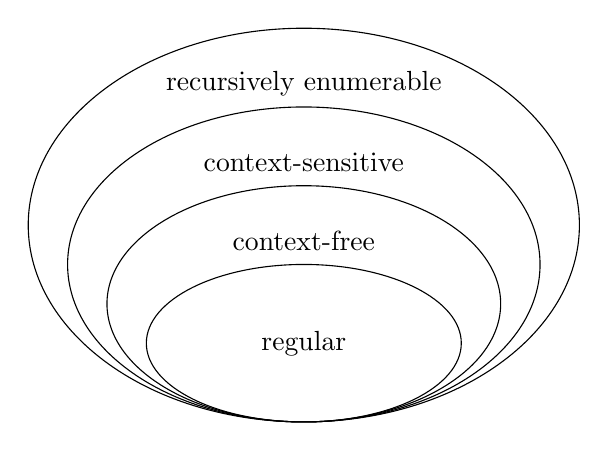
\begin{tikzpicture}
        \draw (0,0) ellipse (2 and 1);
        \draw (0,0.5) ellipse (2.5 and 1.5);
        \draw (0,1) ellipse (3 and 2);
        \draw (0,1.5) ellipse (3.5 and 2.5);

        \node at (0,0) {regular};
        \node at (0,1.3) {context-free};
        \node at (0,2.3) {context-sensitive};
        \node at (0,3.3) {recursively enumerable};
    \end{tikzpicture}
    \caption{Chomsky hierarchy of formal languages}
    \label{fig:chomsky-hierarchy}
\end{figure}


\subsubsection{Practical Implications}
\begin{itemize}
    \item \textbf{Regular Expressions}: Used in text processing (e.g., \texttt{grep}, lexical analyzers) \cite{kernighan1984unix, hopcroft2006introduction}.  
    \item \textbf{Context-Free Grammars}: Define programming language syntax (e.g., Python’s grammar) \cite{chomsky1956three, hopcroft2006introduction}.  
    \item \textbf{Closure Properties}: Enable decidability proofs (e.g., emptiness testing for DFAs) \cite{hopcroft2006introduction}.  
    \item \textbf{Stochastic Models}: Applied in natural language processing and speech recognition for probabilistic pattern matching \cite{rabin1963probabilistic}.  
\end{itemize}

\begin{figure}[h]
    \centering
    \begin{tikzpicture}[->,>=stealth,shorten >=1pt,auto,node distance=2.8cm,
        semithick, state/.style={circle, draw, minimum size=1.5cm}]
    
    \node[state, initial] (q0) {$q_0$};
    \node[state, accepting] (q1) [right of=q0] {$q_1$};
    
    \path 
    (q0) edge [loop above] node {$0$} (q0)
         edge [bend left] node {$1$} (q1)
    (q1) edge [loop above] node {$1$} (q1)
         edge [bend left] node {$0$} (q0);
    \end{tikzpicture}
    \caption{Example DFA recognizing even number of 1s}
    \label{fig:dfa-example}
\end{figure}

\subsubsection{Automata Definition Fundamentals}  
All automata share core structural components \cite{hopcroft2006introduction, chomsky1956three}.  

\begin{definition}[Classical Finite Automaton]
    \label{def:finite-automaton}
    A \textit{finite automaton} is a computational model that processes input symbols to recognize languages. Formally, a finite automaton $M$ is a quintuple $(Q, \Sigma, \delta, q_0, F)$, where:
    \begin{itemize}
        \item {States ($Q$)}: A finite set of configurations representing computational progress \cite{hopcroft2006introduction}. 
        \item {Input Alphabet ($\Sigma$)}: Defined symbols the automaton processes \cite{hopcroft2006introduction}.
        \item {Transition Function ($\delta$)}: Governs state changes based on input \cite{chomsky1956three}:  
        \begin{itemize}
            \item \textit{Deterministic}: $\delta: Q \times \Sigma \to Q$ (e.g., DFA) \cite{hopcroft2006introduction}.  
            \item \textit{Nondeterministic}: $\delta: Q \times \Sigma \to 2^Q$ (e.g., NFA) \cite{rabin1963probabilistic}.  
        \end{itemize}
        \item {Initial State ($q_0 \in Q$)}: The starting configuration \cite{hopcroft2006introduction}. 
        \item {Accept States ($F \subseteq Q$)}: Terminal states indicating successful computation \cite{hopcroft2006introduction}.
    \end{itemize} 
\end{definition}

\noindent\textit{Example}: The DFA in Figure \ref{fig:dfa-example} has:  
\begin{itemize}
    \item $Q = \{q_0, q_1\}$  
    \item $\Sigma = \{0, 1\}$  
    \item $\delta(q_0, 1) = q_1$, $\delta(q_1, 0) = q_0$ \textit{(partial specification)}  
    \item $F = \{q_1\}$ (accepts even number of 1s)  
\end{itemize}
\noindent\textbf{Graphical notation}: 
\begin{itemize}
    \item States: Circles with $q_i$ labels  
        \item Initial state: Arrow pointing to the state ($q_0$)  
        \item Accept states: Double circles ($q_1$ in \ref{fig:dfa-example})  
        \item Transitions: Directed edges labeled with input symbols  
\end{itemize}



\begin{table}[htbp]
    \centering
      \begin{tabular}{@{}lllll@{}}
          \toprule
          \textbf{Automaton} & \textbf{State Memory} & \textbf{Transition Type} & \textbf{Acceptance Condition} \\ \midrule
          DFA & None & Deterministic & Final state membership \cite{hopcroft2006introduction} \\
          NFA & None & Nondeterministic & Existence of accepting path \cite{hopcroft2006introduction} \\
          PDA & Stack & Deterministic/Nondet. & Final state + empty stack \cite{chomsky1956three} \\
          Turing Machine & Tape & Deterministic & Halting in accept state \cite{turing1936computable} \\
          \bottomrule
      \end{tabular}%
    \caption{Automata representation variations}
    \label{tab:automata-variations}
\end{table}

\subsection{Deterministic Finite Automata (DFA)}
\label{subsec:dfa} 

A DFA is a quintuple $M = (Q, \Sigma, \delta, q_0, F)$, where:
\begin{itemize}
    \item $Q$: Finite set of states.
    \item $\Sigma$: Input alphabet.
    \item $\delta: Q \times \Sigma \to Q$: Deterministic transition function.
    \item $q_0 \in Q$: Initial state.
    \item $F \subseteq Q$: Accepting states \cite{hopcroft2006introduction}.
\end{itemize} 

Computation proceeds deterministically: for input $w = a_1 a_2 \dots a_n$, the state evolves as $\delta(q_{i-1}, a_i) = q_i$ \cite{hopcroft2006introduction}. A string $w$ is accepted if $\delta(q_0, w) \in F$. DFAs recognize precisely the regular languages, with expressive power strictly weaker than context-free languages \cite{hopcroft2006introduction}. 

Key properties include:
\begin{itemize}
    \item \textit{Minimization}: Hopcroft's algorithm reduces DFAs to minimal form in $O(n \log n)$ time \cite{hopcroft2006introduction}.
    \item \textit{Emptiness Problem}: Decidable via reachability analysis from $q_0$ to $F$ \cite{hopcroft2006introduction}.
    \item \textit{Pumping Lemma}: For any $L \in \text{REG}$, there exists $p$ such that any $w \in L$ with $\|w\| \geq p$ can be decomposed as $w = xyz$ (with $\|xy\| \leq p$, $\|y\| \geq 1$) such that $xy^i z \in L$ for all $i \geq 0$ \cite{hopcroft2006introduction}.
\end{itemize} 

\newpage
\subsection{\acrfull{nfa}}
\label{subsec:nfa}
\begin{definition}[\gls{nfa}]
    A \gls{nfa} is a quintuple 
    \[
    M = (Q, \Sigma, \delta, q_0, F)
    \]
    where:
    \begin{itemize}
        \item \( Q \) is a finite set of states \cite{kozen1997automata},
        \item \( \Sigma \) is an input alphabet \cite{sudkamp2006languages},
        \item \( \delta: Q \times (\Sigma \cup \{\epsilon\}) \rightarrow 2^Q \) is a nondeterministic transition function \cite{hopcroft2006introduction},
        \item \( q_0 \in Q \) is the initial state,
        \item \( F \subseteq Q \) is the set of accepting states.
    \end{itemize}
\end{definition}

\begin{remark}
Unlike \glspl{dfa}, a \gls{nfa} may have multiple transitions for a given state and input symbol, including transitions on the empty string \(\epsilon\). This nondeterminism allows for multiple computational paths.
\end{remark}

\begin{example}
Figure~\ref{fig:nfa-example} depicts a \gls{nfa} that recognises the language 
\[
L = \{ w \in \{a,b\}^* \mid w \text{ contains the substring } ab \}.
\]
\end{example}

\begin{algorithm}[Subset Construction for \glspl{nfa}]
\label{alg:subset}
To convert an \gls{nfa} \( N = (Q, \Sigma, \delta, q_0, F) \) into an equivalent \gls{dfa} \cite{hopcroft2006introduction, kozen1997automata}:
\begin{enumerate}
    \item Compute the \(\epsilon\)-closure of the initial state: \( S_0 = \epsilon\text{-closure}(\{q_0\}) \).
    \item For each \gls{dfa} state \( S \subseteq Q \) and each input symbol \(\sigma \in \Sigma\), define 
    \[
    \delta_{\text{\gls{dfa}}}(S, \sigma) = \epsilon\text{-closure}\Big(\bigcup_{q \in S} \delta(q, \sigma)\Big).
    \]
    \item Mark \( S \) as accepting if \( S \cap F \neq \emptyset \).
    \item Repeat until no new states are produced.
\end{enumerate}
\end{algorithm}

\begin{observation}
    The subset construction algorithm may produce up to \(2^{|Q|}\) states in the worst case, illustrating a potential state explosion when converting an \gls{nfa} to a \gls{dfa} \cite{sipser2013introduction}.
\end{observation}

\begin{figure}[h]
    \centering  
    \begin{tikzpicture}[shorten >=1pt, node distance=2.5cm, on grid, auto]
        \node[state, initial, initial text={}] (q0) {$q_0$};
        \node[state] (q1) [right=of q0] {$q_1$};
        \node[state, accepting] (q2) [right=of q1] {$q_2$};

        \path[->]
        (q0) edge [loop above] node {$a,b$} (q0)
        (q0) edge node {$a$} (q1)
        (q1) edge node {$b$} (q2);
    \end{tikzpicture}
    \caption{NFA recognizing \( L = \Sigma^*ab \)}
    \label{fig:nfa-example}
\end{figure}

\begin{figure}[h]
    \centering  
    \begin{tikzpicture}[shorten >=1pt, node distance=3cm, on grid, auto]
        \node[state, initial, initial text={}] (A) {$\{q_0\}$};
        \node[state] (B) [right=of A] {$\{q_0, q_1\}$};
        \node[state, accepting] (C) [right=of B] {$\{q_0, q_2\}$};

        \path[->]
        (A) edge [loop below] node {$b$} (A)
        (A) edge node {$a$} (B)
        (B) edge [loop below] node {$a$} (B)
        (B) edge node {$b$} (C)
        (C) edge [bend left] node {$a$} (B)
        (C) edge [bend right] node[swap] {$b$} (A);
    \end{tikzpicture}
    \caption{Equivalent DFA for NFA in Figure~\ref{fig:nfa-example} \cite{hopcroft2006introduction}}
    \label{fig:dfa-conversion}
\end{figure}
\subsection{\glsentrylong{pfa}}
\label{subsec:pfa}

\begin{definition}[\glsentrylong{pfa}]
    A \gls{pfa} is a quintuple 
    \[
    M = (Q, \Sigma, \delta, \pi, F)
    \]
    where:
    \begin{itemize}
        \item \( Q \) is a finite set of states,
        \item \( \Sigma \) is a finite input alphabet,
        \item \( \delta: Q \times \Sigma \times Q \rightarrow [0,1] \) is a probabilistic transition function \cite{rabin1963probabilistic} such that 
        \[
        \sum_{q' \in Q} \delta(q, \sigma, q') = 1 \quad \text{for all } q \in Q \text{ and } \sigma \in \Sigma
        ,\]
        \item \( \pi \in \mathbb{R}^{|Q|} \) is an initial state distribution vector with 
        \[
        \sum_{q \in Q} \pi_q = 1,
        \]
        \item \( F \subseteq Q \) is the set of accepting states.
    \end{itemize}
\end{definition}

\begin{remark}
In a \gls{pfa}, transitions are probabilistic. The acceptance of an input string is determined by whether the cumulative probability of ending in an accepting state exceeds a chosen cut-point.
\end{remark}

\begin{example}
Figure~\ref{fig:pfa-example} illustrates a \gls{pfa} that recognises the language 
\[
L_{\text{maj}} = \{ w \in \{a,b\}^* \mid |w|_a > |w|_b \},
\]
where the acceptance probability is at least \( \frac{2}{3} \).
\end{example}

%TODO: Explain the computation of the acceptance probability
\begin{figure}[ht]
    \centering  
    \begin{tikzpicture}[shorten >=1pt, node distance=3cm, on grid, auto]
        \node[state, initial, initial text={$\pi=1$}] (q0) {$q_0$};
        \node[state, accepting] (q1) [right=of q0] {$q_1$};
        
        \path[->]
        (q0) edge [loop above] node {a(0.6), b(0.4)} (q0)
        (q0) edge [bend left] node {a(0.4), b(0.6)} (q1)
        (q1) edge [loop above] node {a(0.3), b(0.7)} (q1)
        (q1) edge [bend left] node {a(0.7), b(0.3)} (q0);
    \end{tikzpicture}
    \caption{PFA for majority language with probabilistic transitions}
    \label{fig:pfa-example}
\end{figure}

\begin{theorem}[Rabin's Theorem for \glspl{pfa}]
    \label{thm:rabin}
    A \gls{pfa} with an isolated cut-point recognises exactly the class of regular languages \cite{rabin1963probabilistic}.
\end{theorem}

\begin{proposition}
    If a \gls{pfa} employs a non-isolated cut-point (e.g., \(\lambda = 0\)), it may recognise languages beyond the regular class, including some context-sensitive languages \cite{paz1971introduction}.
\end{proposition}

\begin{corollary}
For a \gls{pfa} with a strict cut-point (\(\lambda = 1\)), the recognised language is equivalent to that of a \gls{dfa}.
\end{corollary}

\begin{observation}
    The closure properties of \glspl{pfa} differ from those of classical finite automata. In particular, complementation is not directly achievable unless an isolated cut-point is used \cite{droste2009handbook}.
\end{observation}

\subsection{Two-Way Finite Automata Variants}
\label{subsec:two-way-variants}

Two-way finite automata extend the classical one‐way model by allowing the read head to move in both directions over the input. Although this extra power does not increase the class of recognizable languages, two-way models can be exponentially more succinct than one-way models \cite{sakoda1978nfas, kozen1997automata} and naturally lend themselves to algorithms in several contexts (e.g., in complexity analysis and even quantum models).

\subsubsection{\glsentrylong{2dfa}}
\label{subsubsec:2dfa}

\begin{definition}[\glsentrylong{2dfa}]
A \gls{2dfa} is formally defined as an 8-tuple 
\[
M = (Q, \Sigma, \triangleright, \dashv, \delta, s, t, r),
\]
where:
\begin{itemize}
  \item \(Q\) is a finite set of states,
  \item \(\Sigma\) is a finite input alphabet,
  \item \(\triangleright\) and \(\dashv\) are special symbols called the left and right endmarkers, respectively (with \(\triangleright,\dashv \notin \Sigma\)),
  \item \(\delta: Q \times (\Sigma \cup \{\triangleright, \dashv\}) \to Q \times \{\triangleright,\dashv\}\) is the transition function,
  \item \(s\in Q\) is the start state,
  \item \(t\in Q\) is the unique accept state,
  \item \(r\in Q\) (with \(r\neq t\)) is the unique reject state.
\end{itemize}
In addition, the transition function is assumed to satisfy:
\begin{itemize}
  \item For every state \(q\in Q\), when reading the left endmarker \(\triangleright\), the head always moves in the \(\dashv\) direction; that is, \(\delta(q,\triangleright) = (q', \dashv)\) for some \(q'\in Q\).
  \item Similarly, when reading the right endmarker \(\dashv\), the head always moves in the \(\triangleright\) direction: \(\delta(q,\dashv) = (q', \triangleright)\).
  \item Once the machine reaches the accept state \(t\) (or the reject state \(r\)), it remains there (the transition always maps back to itself) while moving in a fixed direction.
\end{itemize}
\end{definition}

\begin{remark}
The two-way motion allows the automaton to perform multiple passes over the input, which can result in an exponential reduction in the number of states compared to one-way automata, though at the expense of increased operational complexity.
\end{remark}

\begin{example}
    Consider the language 
    \[
    L = \{ w\in \{0,1\}^* \mid \text{the first symbol of } w \text{ equals the last symbol} \}.
    \]
    A \gls{2dfa} for \(L\) operates as follows:
    \begin{enumerate}
      \item Start at \(\triangleright\) and move in the \(\dashv\) direction to read the first symbol, transitioning to a state encoding this symbol (e.g., \(q_a\) for \(a \in \{0,1\}\)).
      \item Continue moving in the \(\dashv\) direction until \(\dashv\) is reached.
      \item Reverse direction and scan in the \(\triangleright\) direction to the last symbol.
      \item Compare the stored symbol (encoded in the current state) with the last symbol. Accept if they match; reject otherwise.
    \end{enumerate}
\end{example}

\begin{observation}
    Although every \gls{2dfa} can be simulated by a \gls{1dfa}, such a simulation may require an exponential increase in the number of states \cite{shepherdson1959reduction}.
\end{observation}

\paragraph{Operational Mechanics}
The two-way motion enables the automaton to make multiple passes over the input, which is particularly useful for verifying properties that depend on both the prefix and the suffix of the input string.

\paragraph{State Complexity and Conversion Algorithms}
For some families of regular languages, \glspl{2dfa} can be exponentially more succinct than their one-way counterparts. Conversion algorithms—such as those proposed by Shepherdson and Kozen—use crossing sequences to simulate two-way behavior in a one-way \gls{dfa}, typically at the cost of exponential state blow-up.

%TODO: enhance the following example
\begin{figure}[ht]
    \centering  
    \begin{tikzpicture}[shorten >=1pt, node distance=2.5cm, on grid, auto]
        \node[state,initial,accepting] (q0) {\(q_0\)};
        \node[state] (q1) [right=of q0] {\(q_1\)};
        \node[state] (q2) [below=of q1] {\(q_2\)};
        \node[state,accepting] (t) [left=of q2] {\(t\)};
        \node[state,rejecting] (r) [right=of q2] {\(r\)};

        \path[->]
            (q0) edge node[above] {\(\triangleright \to \dashv,\, \text{store } a\)} (q1)
            (q1) edge [loop above] node {\(\sigma,\dashv\)} (q1)
            (q1) edge node[right] {\(\dashv \to \triangleright\)} (q2)
            (q2) edge [loop below] node {\(\sigma,\triangleright\)} (q2)
            (q2) edge node[below] {\(\triangleright: a = \text{last?}\)} (t)
            (q2) edge node[above] {\(\triangleright: a \neq \text{last}\)} (r);
    \end{tikzpicture}
    \caption{\gls{2dfa} for \(L = \{w \mid w_1 = w_{|w|}\}\). States encode the first symbol \(a \in \{0,1\}\). Transitions use \(\triangleright/\dashv\) to denote head movement directions and endmarkers.}
    \label{fig:2dfa-example}
\end{figure}

\subsubsection{\glsentrylong{2nfa}}
\label{subsubsec:2nfa}

\begin{definition}[\glsentrylong{2nfa}]
A \gls{2nfa} is defined similarly to a \gls{2dfa} but with a nondeterministic transition function \cite{sakoda1978nfas}. Formally, a \gls{2nfa} is an 8-tuple
\[
M = (Q, \Sigma, \triangleright, \dashv, \delta, s, t, r),
\]
where:
\begin{itemize}
    \item \(Q\) is a finite set of states,
    \item \(\Sigma\) is a finite input alphabet,
    \item \(\triangleright\) and \(\dashv\) are the left and right endmarkers (with \(\triangleright,\dashv \notin \Sigma\)),
    \item \(\delta: Q \times (\Sigma \cup \{\triangleright,\dashv\}) \to 2^{\,Q \times \{\triangleright,\dashv\}}\) is the nondeterministic transition function,
    \item \(s\in Q\) is the start state,
    \item \(t\in Q\) is the unique accept state, and
    \item \(r\in Q\) (with \(r\neq t\)) is the unique reject state.
\end{itemize}
The transition function obeys similar boundary conditions as in the \gls{2dfa} case.
\end{definition}

\begin{remark}
The nondeterminism in a \gls{2nfa} allows it to “guess” important positions within the input and verify them via bidirectional traversal, which can lead to significant state savings compared to deterministic models.
\end{remark}

\begin{example}
Consider the language 
\[
L_{sym} = \{ w \in \{0,1\}^* \mid \text{the first two symbols equal the last two symbols} \}.
\]
A high-level description of a \gls{2nfa} for \(L_{sym}\) is:
\begin{enumerate}
    \item Scan in the \(\dashv\) direction from the left endmarker \(\triangleright\) while nondeterministically guessing the point where comparison will occur.
    \item Upon reaching the right endmarker \(\dashv\), reverse direction.
    \item While moving in the \(\triangleright\) direction, nondeterministically check that the stored first two symbols match the corresponding symbols at the end.
    \item If both comparisons succeed, transition to the accept state \(t\); otherwise, transition to the reject state \(r\).
\end{enumerate}
Figure~\ref{fig:2nfa-example} schematically illustrates this guess-and-check mechanism.
\end{example}

%TODO: enhance the following example
\begin{figure}[ht]
    \centering  
    \begin{tikzpicture}[shorten >=1pt, node distance=2.2cm, on grid, auto]
        \node[state,initial] (q0) {\(q_0\)};
        \node[state] (q1) [right=of q0] {\(q_1\)};
        \node[state] (q2) [right=of q1] {\(q_2\)};
        \node[state,accepting] (qa) [above=of q2] {\(t\)};
        \node[state,rejecting] (qr) [below=of q2] {\(r\)};
        
        \path[->]
            (q0) edge [loop above] node {\(\sigma,\dashv\)} (q0)
            (q0) edge node {\(\triangleright \to \dashv\)} (q1)
            (q1) edge [loop above] node {\(\sigma,\dashv\)} (q1)
            (q1) edge node {\(\dashv \to \triangleright\)} (q2)
            (q2) edge [bend left] node[above left] {\(\sigma,\triangleright\) (guess)} (q0)
            (q2) edge node[right] {\(\sigma = \text{stored?}\)} (qa)
            (q2) edge node[right] {\(\sigma \neq \text{stored}\)} (qr);
    \end{tikzpicture}
    \caption{2NFA for \(L_{\text{sym}} = \{ww^R\}\). The machine nondeterministically guesses the midpoint (via transition \(q_2 \to q_0\)) and verifies symmetry.}
    \label{fig:2nfa-example}
\end{figure}

\begin{observation}
\glspl{2nfa} can be exponentially more succinct than one-way \glspl{dfa}, even though the class of languages they recognise remains the same (i.e., the regular languages).
\end{observation}

\subsubsection{\glsentrylong{2pfa}}
\label{subsubsec:2pfa}

\begin{definition}[\glsentrylong{2pfa}]
A \gls{2pfa} is an 8-tuple
\[
M = (Q, \Sigma, \triangleright, \dashv, \delta, s, t, r),
\]
where:
\begin{itemize}
    \item \(Q\) is a finite set of states,
    \item \(\Sigma\) is a finite input alphabet,
    \item \(\triangleright\) and \(\dashv\) are the left and right endmarkers (with \(\triangleright,\dashv \notin \Sigma\)),
    \item \(\delta: Q \times (\Sigma \cup \{\triangleright,\dashv\}) \to \mathbb{R}_{\ge 0}^{\,Q \times \{\triangleright,\dashv\}}\) is a probabilistic transition function such that
    \[
    \sum_{(q',d)\in Q\times\{\triangleright,\dashv\}} \delta(q,a,q',d) = 1 \quad \text{for all } q \in Q \text{ and } a \in \Sigma \cup \{\triangleright,\dashv\},
    \]
    \item \(s\in Q\) is the start state,
    \item \(t\in Q\) is the unique accept state, and
    \item \(r\in Q\) (with \(r\neq t\)) is the unique reject state.
\end{itemize}
\end{definition}

\begin{remark}
A \gls{2pfa} extends the probabilistic finite automaton by allowing bidirectional head movement. Its transitions are governed by probability distributions, and acceptance is determined by whether the cumulative probability of reaching the accept state exceeds a predetermined cut-point.
\end{remark}

%TODO: link to the previous example, cardinality symbol now is different
\begin{example}
Consider the language 
\[
L_{maj} = \{ w \in \{a,b\}^* \mid \#a(w) > \#b(w) \}.
\]
A \gls{2pfa} for \(L_{maj}\) operates by making probabilistic passes over the input, updating state probabilities, and eventually halting in the accept state \(t\) if the acceptance probability is high enough. Figure~\ref{fig:2pfa-example} provides a schematic illustration of such a machine.
\end{example}

\begin{figure}[ht]
    \centering  
    \begin{tikzpicture}[shorten >=1pt, node distance=2.5cm, on grid, auto]
        \node[state,initial] (q0) {\(q_0\)};
        \node[state] (q1) [right=of q0] {\(q_1\)};
        \node[state,accepting] (q2) [right=of q1] {\(t\)};
        \node[state,rejecting] (qr) [below=of q1] {\(r\)};
        
        \path[->]
            (q0) edge [loop above] node[align=center] 
                {\(a:0.6,\dashv\)\\\(b:0.4,\dashv\)} (q0)
            (q0) edge node[above] {\(\dashv \to \triangleright\)} (q1)
            (q1) edge [loop above] node[align=center] 
                {\(a:0.7,\triangleright\)\\\(b:0.3,\triangleright\)} (q1)
            (q1) edge node[above] {\(\triangleright: \Pr(\text{accept}) \geq 2/3\)} (q2)
            (q1) edge node[below left] {\(\triangleright: \Pr(\text{reject}) \geq 1/3\)} (qr);
    \end{tikzpicture}
    \caption{2PFA for \(L_{\text{maj}} = \{w \mid \#a(w) > \#b(w)\}\). Transitions use probabilistic counts with isolated cut-point \(\lambda = 2/3\), and head movements are indicated by \(\triangleright\) (leftward) and \(\dashv\) (rightward).}
    \label{fig:2pfa-example}
\end{figure}

\begin{theorem}[Dwork-Stockmeyer Theorem]
    \label{thm:2pfa-rabin}
    A \gls{2pfa} with an isolated cut-point recognises exactly the class of regular languages \cite{dwork1990time}.
\end{theorem}

\begin{proposition}
If a \gls{2pfa} employs a non-isolated cut-point (e.g., \(\lambda = 0\)), it may recognise languages beyond the regular class.
\end{proposition}

%TODO: add these explainations to the 1PFA too.
\begin{corollary}
For a \gls{2pfa} with a strict cut-point (\(\lambda = 1\)), the recognised language is equivalent to that of a \gls{dfa}.
\end{corollary}

\subsubsection{Comparative Analysis of Two-Way Models}
\label{subsubsec:two-way-comparison}

%TODO: check the correctness of the following table and specify 2PFA. Moreover, add comparison summary also for 1 way models.

\begin{table}[ht]
    \label{tab:two-way-comparison}
    \centering
    \begin{tabular}{|l|c|c|c|c|l|}
        \hline
        \textbf{Model} & \textbf{Language Class} & \textbf{Time} & \textbf{Space} & \textbf{States} & \textbf{Key Reference} \\ 
        \hline
        \gls{2dfa}  & REG & \(O(n^2)\) & \(O(1)\) & \(2^{\Theta(n)}\) & \cite{shepherdson1959reduction} \\
        \gls{2nfa}  & REG & \(O(n)\) & \(O(1)\) & \(O(1)\) & \cite{sakoda1978nfas} \\
        \gls{2pfa}  & REG (isolated cut) & \(O(n^3)\) & \(O(\log n)\) & \(O(1)\) & \cite{dwork1990time} \\
        \hline
    \end{tabular}
    \caption{Comparative analysis of two-way automata models}
\end{table}

\begin{remark}
The comparative analysis illustrates that while all two-way automata recognise only regular languages, the two-way models often achieve significant advantages in state complexity and, in some cases, time complexity, compared to their one-way counterparts.
\end{remark} 


% \subsection{Key Theorems}
% \label{subsec:key-theorems} 

% \begin{enumerate}
%     \item \textit{Kleene's Theorem}: A language is regular if and only if it is recognized by a DFA/NFA or described by a regular expression \cite{hopcroft2006introduction}.
%     \item \textit{Subset Construction Theorem}: Every NFA can be converted to an equivalent DFA, with up to $2^n$ states \cite{hopcroft2006introduction}.
%     \item \textit{Myhill-Nerode Theorem}: Characterizes $\text{REG}$ via string indistinguishability, forming the basis for DFA minimization \cite{hopcroft2006introduction}.
%     \item \textit{Rabin's Theorem}: PFAs recognize stochastic languages, a strict superset of $\text{REG}$ \cite{rabin1963probabilistic}.
%     \item \textit{Sipser's Theorem}: 2PFAs recognize $\text{REG}$ in logarithmic space but require exponential time for non-regular languages \cite{sipser1980halting}.
% \end{enumerate} 

% These theorems collectively delineate the boundaries of classical finite automata, setting the stage for quantum extensions in subsequent chapters. 


\newpage
\section{Quantum Mechanics Foundations}
\label{sec:quantum-foundations}

This section establishes the quantum mechanical principles that underpin quantum automata theory. We emphasize both the mathematical formalism and the conceptual distinctions from classical systems. In what follows, we review the basic postulates of quantum mechanics, elaborate on the structure and evolution of quantum states, and discuss measurement, decoherence, and their computational implications.



\subsection{Qubits and Quantum States}
\label{subsec:qubits}

\begin{definition}[Qubit]
A \emph{\gls{qubit}} is the fundamental unit of quantum information. It is represented as a normalised vector in a two-dimensional complex Hilbert space,
\[
\mathcal{H} = \mathbb{C}^2.
\]
\end{definition}

\begin{notation}[Computational Basis]
The standard (computational) basis states for a qubit are defined as
\[
|0\rangle = \begin{pmatrix} 1 \\ 0 \end{pmatrix}, \quad |1\rangle = \begin{pmatrix} 0 \\ 1 \end{pmatrix}.
\]
\end{notation}

\begin{definition}[General Qubit State]
A general state of a \gls{qubit} is given by
\[
|\psi\rangle = \alpha|0\rangle + \beta|1\rangle, \quad \text{with } |\alpha|^2 + |\beta|^2 = 1,
\]
where \(\alpha,\beta \in \mathbb{C}\) are the \emph{probability amplitudes}.
\end{definition}

\begin{remark}
Global phase factors—i.e. multiplying the state by an overall phase \(e^{i\gamma}\)—do not affect the physical properties of the qubit.
\end{remark}

\begin{example}[Bloch Sphere Representation]
  Any pure state of a \gls{qubit} can be written in the form
  \[
  |\psi\rangle = \cos\frac{\theta}{2}|0\rangle + e^{i\phi}\sin\frac{\theta}{2}|1\rangle,
  \]
  with \(\theta \in [0,\pi]\) and \(\phi \in [0,2\pi)\). Figure~\ref{fig:bloch_sphere} illustrates the \textbf{Bloch sphere} representation of a qubit \cite{nielsen2010quantum}.
\end{example}

\begin{figure}[h]
  \centering
  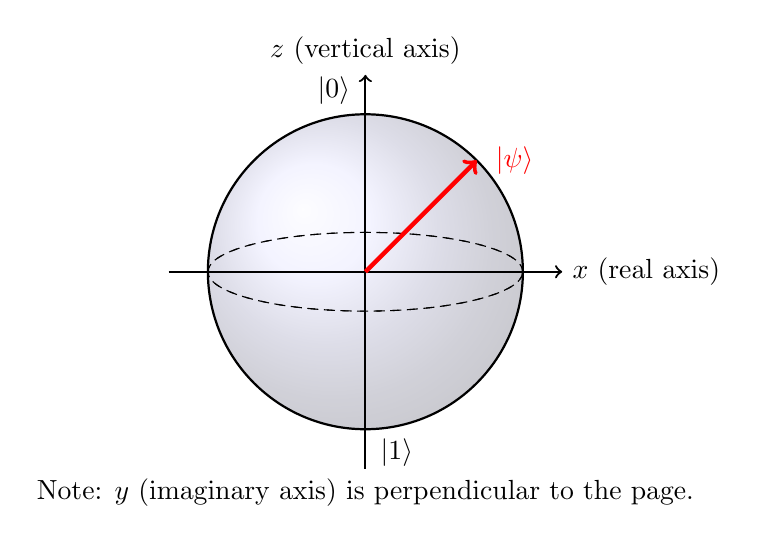
\begin{tikzpicture}[scale=1]
    % Draw sphere outline with shading
    \shade[ball color=blue!20, opacity=0.3] (0,0) circle (2cm);
    \draw[thick] (0,0) circle (2cm);
    
    % Draw equator as a dashed ellipse (horizontal cross-section)
    \draw[dashed] (0,0) ellipse (2cm and 0.5cm);
    
    % Draw meridian arcs (vertical cross-sections)
    \draw[dashed] (-2,0) arc (180:0:2cm and 0.5cm);
    \draw[dashed] (2,0) arc (0:-180:2cm and 0.5cm);
    
    % Axes: x and z
    \draw[->, thick] (-2.5,0) -- (2.5,0) node[right] {$x$ (real axis)};
    \draw[->, thick] (0,-2.5) -- (0,2.5) node[above] {$z$ (vertical axis)};
    
    % Mark north and south poles with horizontal shift
    \node[above, xshift=-0.4cm] at (0,2) {\(|0\rangle\)};
    \node[below, xshift=0.4cm] at (0,-2) {\(|1\rangle\)};
    
    % Bloch vector in the x-z plane
    \draw[->, red, ultra thick] (0,0) -- (1.414,1.414) node[right] {\(\;|\psi\rangle\)};
    
    % Note for y axis
    \node at (0,-2.8) {Note: \(y\) (imaginary axis) is perpendicular to the page.};
  \end{tikzpicture}
  \caption{Enhanced Bloch sphere representation of a \gls{qubit} with adjusted labels.}
  \label{fig:bloch_sphere}
  \end{figure}

\begin{observation}
  For multi-qubit systems, the overall state space is given by the tensor product of individual qubit spaces. For instance, a two-qubit system is described by
  \[
  |\psi\rangle = \sum_{i,j \in \{0,1\}} \alpha_{ij}\, |i\rangle \otimes |j\rangle, \quad \sum_{i,j} |\alpha_{ij}|^2 = 1.
  \]
  This exponential scaling of the state space underpins the potential of quantum parallelism \cite{nielsen2010quantum}.
\end{observation}



\subsection{Superposition and Entanglement}
\label{subsec:superposition}

\textbf{Superposition} enables parallel computation. The Hadamard gate ($H$) creates uniform superpositions:
\[
H|0\rangle = \frac{|0\rangle + |1\rangle}{\sqrt{2}}, \quad H|1\rangle = \frac{|0\rangle - |1\rangle}{\sqrt{2}}.
\]

\textbf{Entanglement} arises in multi-qubit states that cannot be factored. The Bell states are maximally entangled:
\[
|\Phi^+\rangle = \frac{|00\rangle + |11\rangle}{\sqrt{2}}, \quad |\Phi^-\rangle = \frac{|00\rangle - |11\rangle}{\sqrt{2}},
\]
\[
|\Psi^+\rangle = \frac{|01\rangle + |10\rangle}{\sqrt{2}}, \quad |\Psi^-\rangle = \frac{|01\rangle - |10\rangle}{\sqrt{2}}.
\]

\begin{figure}[h]
\centering
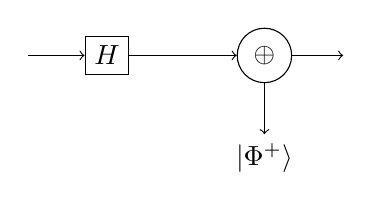
\begin{tikzpicture}
  \node[draw,rectangle] (h) at (0,0) {$H$};
  \node[draw,circle] (cnot) at (2,0) {$\oplus$};
  \draw[->] (-1,0) -- (h);
  \draw[->] (h) -- (cnot);
  \draw[->] (cnot) -- (3,0);
  \draw[->] (cnot) -- (2,-1) node[below] {$|\Phi^+\rangle$};
\end{tikzpicture}
\caption{Quantum circuit generating the Bell state $|\Phi^+\rangle$.}
\label{fig:bell_circuit}
\end{figure}

Entanglement is critical for quantum teleportation \cite{bennett1993teleporting} and enables exponential speedups in algorithms like Shor's \cite{shor1999polynomial}.

\subsection{Quantum Gates and Circuits}
\label{subsec:gates}

Quantum gates are the building blocks of quantum circuits. They are represented by \emph{unitary operators} \(U\) (i.e. \(U^\dagger U = I\)) that govern the evolution of quantum states. Key single-qubit gates include:
\begin{itemize}
    \item \textbf{Pauli-X (bit-flip):} 
    \[
    X = \begin{pmatrix} 0 & 1 \\ 1 & 0 \end{pmatrix},
    \]
    which acts as \(X|0\rangle = |1\rangle\) and \(X|1\rangle = |0\rangle\).
    \item \textbf{Hadamard (creating superpositions):}
    \[
    H = \frac{1}{\sqrt{2}}\begin{pmatrix} 1 & 1 \\ 1 & -1 \end{pmatrix}.
    \]
    \item \textbf{Phase shift:}
    \[
    R_\phi = \begin{pmatrix} 1 & 0 \\ 0 & e^{i\phi} \end{pmatrix}.
    \]
\end{itemize}

Two-qubit gates, such as the \textbf{Controlled-NOT (CNOT) gate}, introduce entanglement. The CNOT gate acts on a pair of qubits as
\[
\text{CNOT}|a\rangle|b\rangle = |a\rangle|a \oplus b\rangle,
\]
where \(\oplus\) denotes addition modulo 2.

Quantum circuits decompose complex algorithms into sequences of gate operations. A universal gate set (e.g., \(\{H, T, \text{CNOT}\}\)) can approximate any unitary operation to arbitrary precision, forming the basis for the quantum circuit model.

Figure~\ref{fig:deutsch_circuit} shows an example quantum circuit used in the Deutsch-Jozsa algorithm, illustrating the interplay of Hadamard gates and entangling operations.

\begin{figure}[h]
\centering
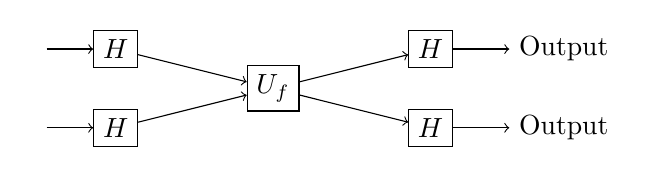
\begin{tikzpicture}[node distance=1.8cm, auto]
    \node (in1) at (0,0) {};
    \node (in2) at (0,-1) {};
    \node[draw, rectangle] (H1) at (1,0) {$H$};
    \node[draw, rectangle] (H2) at (1,-1) {$H$};
    \node[draw, rectangle] (Uf) at (3, -0.5) {\(U_f\)};
    \node[draw, rectangle] (H3) at (5,0) {$H$};
    \node[draw, rectangle] (H4) at (5,-1) {$H$};
    \draw[->] (in1) -- (H1);
    \draw[->] (in2) -- (H2);
    \draw[->] (H1) -- (Uf);
    \draw[->] (H2) -- (Uf);
    \draw[->] (Uf) -- (H3);
    \draw[->] (Uf) -- (H4);
    \draw[->] (H3) -- ++(1,0) node[right] {Output};
    \draw[->] (H4) -- ++(1,0) node[right] {Output};
\end{tikzpicture}
\caption{Quantum circuit for the Deutsch-Jozsa algorithm.}
\label{fig:deutsch_circuit}
\end{figure}

\subsection{Measurement and Probabilistic Outcomes}
\label{subsec:measurement}

Measurement collapses a state to a basis vector. For $|\psi\rangle = \sum_i \alpha_i|i\rangle$, the probability of outcome $i$ is $|\alpha_i|^2$ (Born rule). For example, measuring $|\Phi^+\rangle$ in the computational basis yields $|00\rangle$ or $|11\rangle$ with 50\% probability each.

\begin{table}[h]
\centering
\caption{Measurement outcomes for $|\Phi^+\rangle$.}
\label{tab:bell_measurement}
\begin{tabular}{|c|c|}
\hline
\textbf{Outcome} & \textbf{Probability} \\ \hline
$|00\rangle$      & 50\%                \\ \hline
$|11\rangle$      & 50\%                \\ \hline
\end{tabular}
\end{table}

Mixed states are described by density matrices $\rho = \sum_i p_i |\psi_i\rangle\langle\psi_i|$. This formalism is essential for open quantum systems \cite{breuer2002theory}.
\subsection{Decoherence and Open Systems}
\label{subsec:decoherence}

Decoherence arises from environment interactions, modeled by the Lindblad equation:
\[
\frac{d\rho}{dt} = -\frac{i}{\hbar}[H, \rho] + \sum_k \left( L_k \rho L_k^\dagger - \frac{1}{2}\{L_k^\dagger L_k, \rho\} \right),
\]
where $L_k$ are Lindblad operators \cite{breuer2002theory}. Common noise models include:
- \textbf{Amplitude damping}: Energy loss to the environment.
- \textbf{Phase damping}: Loss of phase coherence.

\begin{figure}[h]
\centering
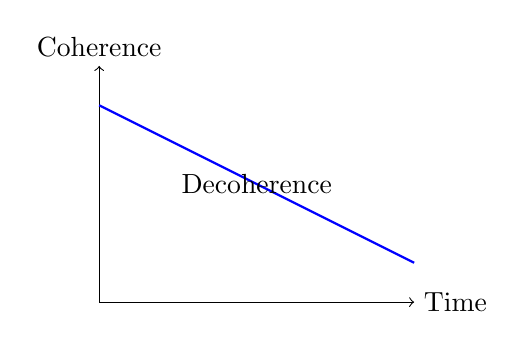
\begin{tikzpicture}
  \draw[->] (0,0) -- (4,0) node[right] {Time};
  \draw[->] (0,0) -- (0,3) node[above] {Coherence};
  \draw[thick,blue] (0,2.5) -- (4,0.5);
  \node at (2,1.5) {Decoherence};
\end{tikzpicture}
\caption{Decoherence reduces quantum state fidelity over time.}
\label{fig:decoherence}
\end{figure}

Quantum error correction codes, like the Shor code \cite{shor1995scheme}, mitigate decoherence by encoding logical qubits into multiple physical qubits. 

\subsection{Additional Remarks: Unitary Evolution and Quantum Dynamics}
\label{subsec:unitary_evolution}

\begin{definition}[Unitary Evolution]
In a closed quantum system, the state evolution is governed by the Schrödinger equation,
\[
i\hbar \frac{d}{dt} |\psi(t)\rangle = H |\psi(t)\rangle,
\]
where \(H\) is the Hamiltonian. The solution to this equation is given by
\[
|\psi(t)\rangle = U(t)|\psi(0)\rangle, \quad \text{with } U(t)=e^{-iHt/\hbar},
\]
where \(U(t)\) is a unitary operator.
\end{definition}

\begin{remark}
Unitary evolution is reversible and forms the basis for the operation of quantum circuits, where continuous evolution is discretized into sequences of quantum gates.
\end{remark}

\begin{theorem}[No-Cloning Theorem]
    Let \(\mathcal{H}\) be a Hilbert space with \(\dim \mathcal{H} \ge 2\). There is no unitary operator \(U\) such that for all states \(|\psi\rangle \in \mathcal{H}\) the following holds:
    \[
    U\big(|\psi\rangle \otimes |0\rangle\big) = |\psi\rangle \otimes |\psi\rangle.
    \]
\end{theorem}

\begin{observation}
    The \textbf{no-cloning theorem} states that it is impossible to create an exact copy of an arbitrary unknown quantum state. This fundamental principle has significant implications for quantum information processing and quantum cryptography.
    The no-cloning theorem ensures that quantum information cannot be perfectly replicated, which underpins the security of many quantum cryptographic protocols.
\end{observation}    
